% Options for packages loaded elsewhere
\PassOptionsToPackage{unicode}{hyperref}
\PassOptionsToPackage{hyphens}{url}
%
\documentclass[
]{article}
\usepackage{amsmath,amssymb}
\usepackage{iftex}
\ifPDFTeX
  \usepackage[T1]{fontenc}
  \usepackage[utf8]{inputenc}
  \usepackage{textcomp} % provide euro and other symbols
\else % if luatex or xetex
  \usepackage{unicode-math} % this also loads fontspec
  \defaultfontfeatures{Scale=MatchLowercase}
  \defaultfontfeatures[\rmfamily]{Ligatures=TeX,Scale=1}
\fi
\usepackage{lmodern}
\ifPDFTeX\else
  % xetex/luatex font selection
\fi
% Use upquote if available, for straight quotes in verbatim environments
\IfFileExists{upquote.sty}{\usepackage{upquote}}{}
\IfFileExists{microtype.sty}{% use microtype if available
  \usepackage[]{microtype}
  \UseMicrotypeSet[protrusion]{basicmath} % disable protrusion for tt fonts
}{}
\makeatletter
\@ifundefined{KOMAClassName}{% if non-KOMA class
  \IfFileExists{parskip.sty}{%
    \usepackage{parskip}
  }{% else
    \setlength{\parindent}{0pt}
    \setlength{\parskip}{6pt plus 2pt minus 1pt}}
}{% if KOMA class
  \KOMAoptions{parskip=half}}
\makeatother
\usepackage{xcolor}
\usepackage[margin=1in]{geometry}
\usepackage{longtable,booktabs,array}
\usepackage{calc} % for calculating minipage widths
% Correct order of tables after \paragraph or \subparagraph
\usepackage{etoolbox}
\makeatletter
\patchcmd\longtable{\par}{\if@noskipsec\mbox{}\fi\par}{}{}
\makeatother
% Allow footnotes in longtable head/foot
\IfFileExists{footnotehyper.sty}{\usepackage{footnotehyper}}{\usepackage{footnote}}
\makesavenoteenv{longtable}
\usepackage{graphicx}
\makeatletter
\def\maxwidth{\ifdim\Gin@nat@width>\linewidth\linewidth\else\Gin@nat@width\fi}
\def\maxheight{\ifdim\Gin@nat@height>\textheight\textheight\else\Gin@nat@height\fi}
\makeatother
% Scale images if necessary, so that they will not overflow the page
% margins by default, and it is still possible to overwrite the defaults
% using explicit options in \includegraphics[width, height, ...]{}
\setkeys{Gin}{width=\maxwidth,height=\maxheight,keepaspectratio}
% Set default figure placement to htbp
\makeatletter
\def\fps@figure{htbp}
\makeatother
\setlength{\emergencystretch}{3em} % prevent overfull lines
\providecommand{\tightlist}{%
  \setlength{\itemsep}{0pt}\setlength{\parskip}{0pt}}
\setcounter{secnumdepth}{5}
\ifLuaTeX
  \usepackage{selnolig}  % disable illegal ligatures
\fi
\usepackage{bookmark}
\IfFileExists{xurl.sty}{\usepackage{xurl}}{} % add URL line breaks if available
\urlstyle{same}
\hypersetup{
  pdftitle={Reviewer1\_MovementQ},
  pdfauthor={Sophie Wulfing},
  hidelinks,
  pdfcreator={LaTeX via pandoc}}

\title{Reviewer1\_MovementQ}
\author{Sophie Wulfing}
\date{2024-06-23}

\begin{document}
\maketitle

\begin{longtable}[]{@{}llll@{}}
\caption{\label{tab:DefaultParamTable}(ref:defaultparamtable) \label{DefaultParamTable}}\tabularnewline
\toprule\noalign{}
Parameter & Population 1 & Population 2 & Definition \\
\midrule\noalign{}
\endfirsthead
\toprule\noalign{}
Parameter & Population 1 & Population 2 & Definition \\
\midrule\noalign{}
\endhead
\bottomrule\noalign{}
\endlastfoot
r & 0.16 & 0.16 & Fish net growth \\
s & 0.8 & 0.8 & Supply and demand \\
h & 0.25 & 0.25 & Harvesting efficiency \\
k & 0.17 & 0.17 & Rate of sampling opinions or social interaction \\
\(\omega\) & 1.44 & 1.44 & Conservation cost \\
c & 0.5 & 0.5 & Rarity valuation \\
d & 0.3 & 0.3 & Strength of social influence (within population) \\
m & 0.01 & 0.01 & Fish movement (from opposite patch) \\
\(\rho\) & 0.01 & 0.01 & Strength of social influence (from opposite population) \\
\end{longtable}

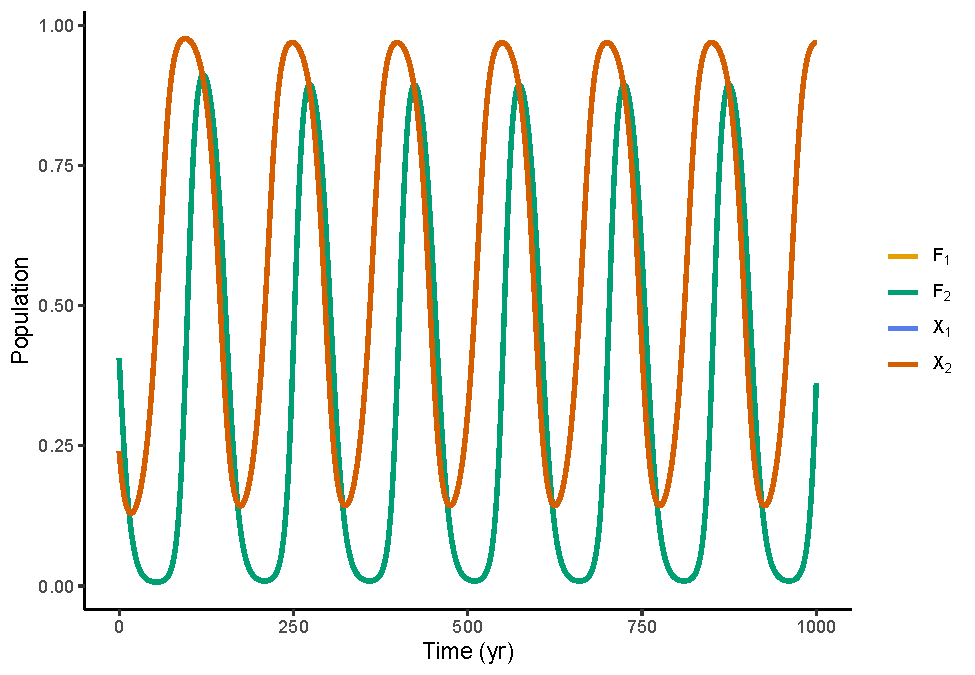
\includegraphics{ReviewerMovementTest_files/figure-latex/Bauch.Coupled-1.pdf}



\begin{figure}
\centering
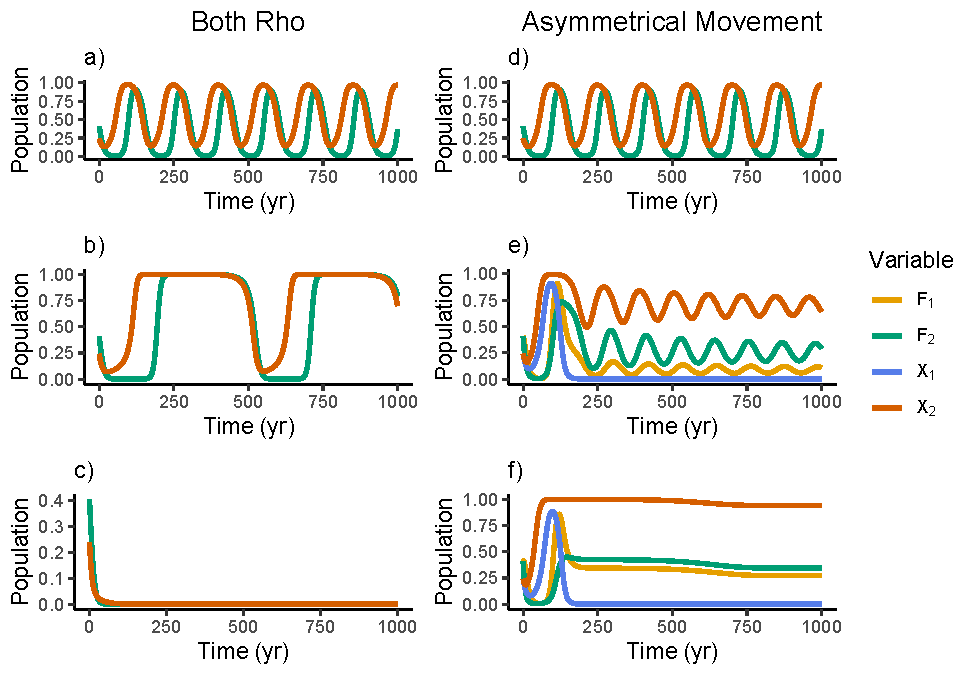
\includegraphics{ReviewerMovementTest_files/figure-latex/MovementBothRho-1.pdf}
\caption{\label{fig:MovementBothRho}In graphs a), b), and c), both \(\rho_1\) and \(\rho_2\) were set to 0.01, 0.25, and 0.5, respectively. The corresponding graphs show the dynamics of these models with the new parameterizations. d), e), and f) show the changes in model dynamics when \(m_2\) is held at 0.01 and only \(m_1\) (the movement of resources from patch 2 to patch 1) is increased by 0.01, 0.05, and 0.1, respectively. \label{MovementBothRho}}
\end{figure}



\begin{figure}
\centering
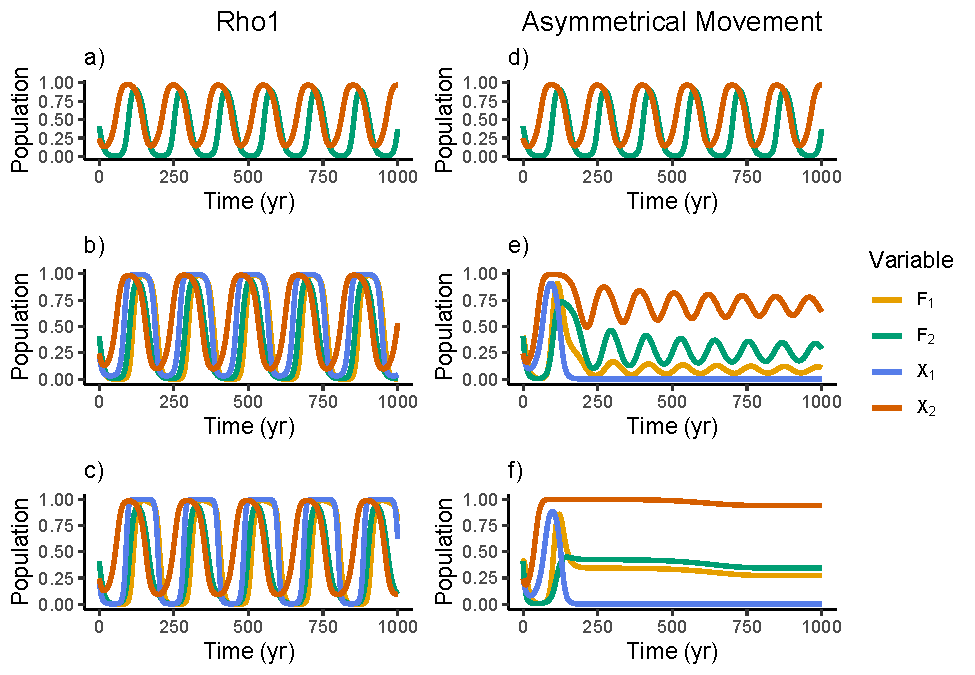
\includegraphics{ReviewerMovementTest_files/figure-latex/MovementOneRho-1.pdf}
\caption{\label{fig:MovementOneRho}In graphs a), b), and c), \(\rho_1\) was set to 0.01, 0.5, and 1, respectively. The corresponding graphs show the dynamics of these models with the new parameterizations. d), e), and f) show the changes in model dynamics when \(m_2\) is held at 0.01 and only \(m_1\) (the movement of resources from patch 2 to patch 1) is increased by 0.01, 0.05, and 0.1, respectively. \label{MovementOneRho}}
\end{figure}

\newpage

\section{Looking at rho params in symmetrical case}\label{looking-at-rho-params-in-symmetrical-case}



\begin{figure}
\centering
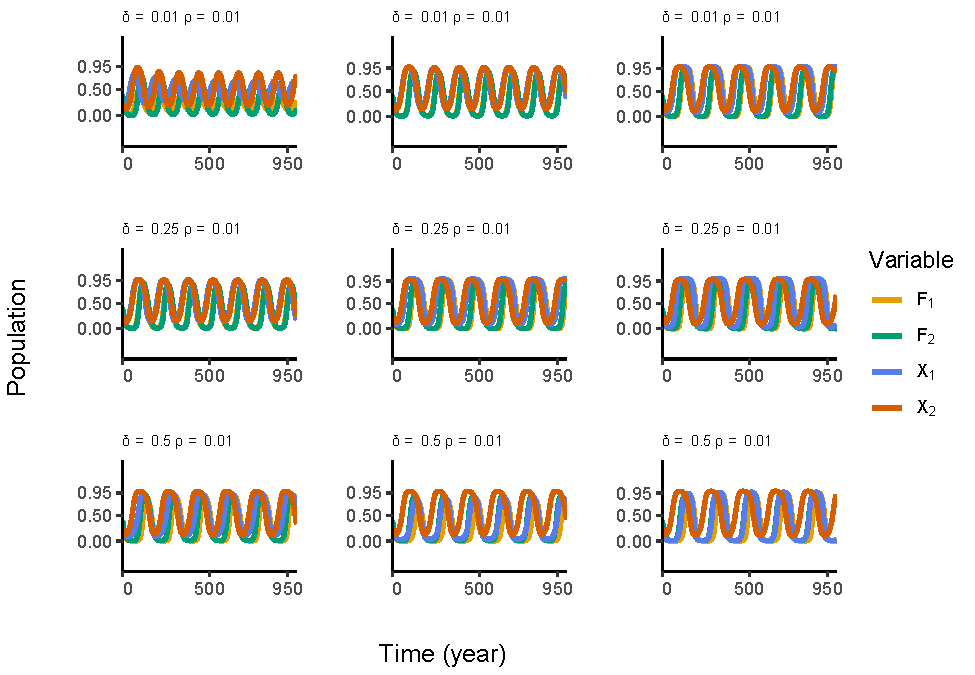
\includegraphics{ReviewerMovementTest_files/figure-latex/influenceAsym-1.pdf}
\caption{\label{fig:influenceAsym}Listening to yourself (\(d_1\)) vs other pop (\(\rho_1\)) \label{influenceAsym}}
\end{figure}

\end{document}
